\documentclass[aspectratio=169,10pt]{beamer}
\usepackage{booktabs}
\usepackage{graphicx}
\graphicspath{{figures/dataset_slides/}}
\setbeamertemplate{navigation symbols}{}
\setbeamertemplate{footline}[frame number]
\newcommand{\mmh}{\,mm\,h$^{-1}$}
\newcommand{\code}[1]{\texttt{\small #1}}

\title{A screened OPERA dataset for km-scale extreme precipitation}
\subtitle{From the v1 patch set to the v4 screen: what was found, built and decided}
\author{Filippo Quarenghi}
\date{7 October 2026}

\begin{document}

\begin{frame}
  \titlepage
\end{frame}

\begin{frame}{Outline}
  \tableofcontents
\end{frame}

% ---------------------------------------------------------------------------
\section{Why the dataset was rebuilt}

\begin{frame}{The v1 patch set could not support the tail claims}
  \small
  \begin{itemize}
    \item \textbf{Splits leak.} Patches were shuffled individually over 2023-08 to 2024-10 on
      the same 79 tile locations. For 100\% of test patches (including max $\ge$ 89\mmh) a
      train patch exists at the same timestamp and on the same tile within $\pm$1\,h. Test
      scores are interpolation scores.
    \item \textbf{The DEM channel was N--S mirrored.} The DEM GeoTIFF is north-first and the
      precipitation stores south-first; both were sliced with the same index. 20/20 test
      patches match the mirrored slice (e.g.\ correlation $-0.32$ with the true terrain).
    \item \textbf{The tail was censored and holed.} Preprocessing set every value $>$150\mmh\
      to \emph{zero}, not to 150. The 435 original days had also been capped at 150\mmh\
      upstream.
    \item \textbf{The tail was contaminated.} On the test split the share of patches whose
      mass sits in a few pixels ($\bar{x}/x_{\max} < 10^{-3}$) \emph{rises} with the
      threshold: 25.9\% at 31, 29.3\% at 89\mmh. Real cells wet more area as they intensify.
    \item \textbf{Only 15 months.} Too little to hold out unseen extremes.
  \end{itemize}
  \vspace{2mm}
  Fixes: the DEM is looked up by patch position (\code{src.data.geo.dem\_patch}); everything
  else needs a new dataset built from the full archive.
\end{frame}

% ---------------------------------------------------------------------------
\section{The raw archive}

\begin{frame}{The OPERA archive on disk}
  \small
  \begin{itemize}
    \item Source: EUMETNET open radar data, anonymous S3 bucket \code{openradar-archive}
      (\code{scripts/data/fetch\_opera\_archive.py}). Rain rate + quality index (QIND),
      ODIM HDF5, LAEA grid $2200\times1900$, 2\,km, 15\,min.
    \item \textbf{4,683 days complete}, 2012-09-04 to 2025-10-22 (the other 114 calendar days
      have no data), 1.2\,TB. 2025-10-23 to 2026-09-22 (334 days) stopped on the user quota.
    \item The 435 original 2023--24 stores (capped at 150\mmh, no QIND) were replaced by
      archive refetches; they agree 100\% below 149\mmh\ (footprint IoU 0.9999).
    \item \textbf{The raw field is dirty.} On 2018-06-15, 52 of 96 composites have a maximum
      above 500\mmh; the peak is 13,072\mmh. Offenders are isolated pixels.
    \item \textbf{Product breaks} to watch when pooling years: late 2015 (blockage correction,
      cloud mask), 2017-09-29 (log $\to$ linear compositing), \textbf{2024-07-05} (ODYSSEY
      $\to$ NIMBUS).
  \end{itemize}
\end{frame}

\begin{frame}{ODYSSEY vs NIMBUS: the same days, two products}
  \small
  ODYSSEY composites the scans of a 15-min window; NIMBUS takes the lowest-elevation scan at
  the nominal time. Paired comparison on the 101 days held in both (2,407 frames, 97,682 wet
  tiles):
  \vspace{2mm}

  \centering
  \begin{tabular}{lc}
    \toprule
    quantity & NIMBUS / ODYSSEY \\
    \midrule
    wet area $\ge$ 0.1 / 1\mmh & 0.71 / 0.99 \\
    exceedance $\ge$ 10 / 31 / 89\mmh & 1.36 / 1.44 / 2.4 \\
    wet-pixel p50 / p90 / p99 & 1.44 / 1.38 / 1.45 \\
    perimeter at 10--31\mmh & $\approx$1.8 \\
    spectral power at 128 / 32 / 8 / 4\,km & 1.25 / 1.42 / 3.1 / 6.2 \\
    +15\,min correlation & 0.41 $\to$ 0.26 \\
    \bottomrule
  \end{tabular}
  \vspace{2mm}

  \raggedright
  NIMBUS fields are more intense, rougher and more fragmented at small scales.
  \textbf{Decision (DECISIONS §18):} train/val/test are ODYSSEY only; NIMBUS is a separate
  product-shift test split (\code{nimbus}, \code{events\_nimbus}).
\end{frame}

% ---------------------------------------------------------------------------
\section{v2: cleaning, leak-free splits, events}

\begin{frame}{v2 pipeline (\code{scripts/dataset\_v2/})}
  \small
  \begin{enumerate}
    \item \textbf{Scan.} Per-year clutter climatology; every frame cleaned
      (\code{src/data/cleaning.py}: drizzle floor, static-clutter and spike \emph{repair},
      no zeroing above 150\mmh); every fully covered $128\times128$ tile described.
    \item \textbf{Splits} (\code{make\_splits.py}):
      \begin{itemize}
        \item whole ISO weeks drawn per calendar month, 1-day buffers $\Rightarrow$ train is
          $\ge$ 2 days from val/test;
        \item 26 catalogued events (ECMWF, MeteoSwiss, DWD, ESSL, AEMET, Météo-France
          studies) forced into test;
        \item tiles rejected if unphysical ($>$500\mmh\ after repair) or an RLAN ray;
        \item stratified sample of 3M patches with per-row inclusion weights.
      \end{itemize}
    \item \textbf{Store}, gamma targets, \code{check\_datasets.py}.
  \end{enumerate}
  \vspace{1mm}
  Subsets: \code{full\_*}, \code{light\_*} (25\%), \code{extremes\_*} (max $\ge$ 31\mmh),
  \code{events\_test} (every tile of every event).
  \vspace{1mm}

  \textbf{Built 2026-10-01/02:} train 1,977,908 / val 251,667 / test 282,684 / nimbus 487,743
  patches on 3,168 / 404 / 463 / 801 days. All checks passed. The log1p scaler moves from 5.02
  to $\approx$6.2 because nothing is zeroed any more.
\end{frame}

\begin{frame}{Audit flags and consistently bad radars}
  \small
  \begin{itemize}
    \item \textbf{Temporal support:} a cell $\ge$ 10\mmh\ with no echo $\ge$ 1\mmh\ within
      30\,km at $t\pm15$\,min.
    \item \textbf{Range rings:} invisible in single frames, but circles in the per-year
      $\ge$ 31\mmh\ frequency. Stevns and Sindal (DK, $\sim$234\,km, 2013--17), Ikaalinen and
      Vimpeli (FI, 2012); none after the 2017-09-29 compositing change.
    \item \textbf{Bad radars} (whole archive, relative to the 5 nearest radars): 14 of 261
      consistently bad, e.g.\ Bollène (clutter, 15/15 years), Teolo ($>$500\mmh), Ängelholm,
      Stevns, Sindal (unsupported maxima), Berlin (ring 2013--15).
    \item The first ranking flagged 204 of 246 radars. Three bugs: a zero 95th percentile used
      as outlier bound; duplicate current/archive database entries splitting a site; 16 sites
      without ODIM code dropped by a \code{groupby}.
  \end{itemize}
\end{frame}

% ---------------------------------------------------------------------------
\section{Validation against rain gauges}

\begin{frame}{Gauge data and design}
  \small
  \begin{itemize}
    \item Independent truth: 10-min gauges from DWD (1,454) and MeteoSwiss SwissMetNet (281);
      12.1M station-frames on 4,968 days.
    \item Gauge QC on the gauges alone: fault codes ($>$50\,mm/10\,min), stuck runs,
      isolated bursts with no rain within 30\,km. 230 of 84.7M wet values masked.
    \item Two questions, by raw intensity bin and per rule:
      \begin{itemize}
        \item \emph{presence}: did the gauge see rain ($\ge$ 1\mmh) under the pixel?
        \item \emph{values}: exceedance ratio
          $\rho(u) = N(\text{radar} \ge u) / N(\text{gauge} \ge u)$ over the same
          station-frames, no conditioning on either side. A flat $\rho$ means the tail has the
          right shape; its level mixes point-vs-2\,km and instantaneous-vs-10-min offsets.
      \end{itemize}
    \item The radar frame matches the gauge interval 10--20\,min later (log-rate correlation
      0.29--0.47).
  \end{itemize}
\end{frame}

\begin{frame}{Presence: which rules remove rain?}
  \footnotesize
  Share of pixels with gauge $\ge$ 1\mmh, by raw intensity:
  \vspace{1mm}

  \centering
  \begin{tabular}{lccccc}
    \toprule
    class & [10,31) & [31,89) & [89,150) & [150,500) & $\ge$500 \\
    \midrule
    untouched & 0.91 & 0.92 & 0.91 & 0.90 & -- \\
    no temporal support & 0.01 & 0.01 & 0.00 & 0.00 & 0.01 \\
    on range ring & 0.82 & 0.50 & 0.00 & 0.00 & 0.00 \\
    spike repaired & 0.13 & 0.24 & 0.24 & 0.26 & 0.00 \\
    tile rejected: unphysical & 0.81 & 0.74 & 0.55 & 0.10 & 0.05 \\
    tile rejected: ray & 0.73 & 0.57 & 0.25 & 0.00 & 0.06 \\
    \bottomrule
  \end{tabular}
  \vspace{2mm}

  \raggedright\small
  \begin{itemize}
    \item Temporal support is the cleanest rule; rings carry real rain below 31\mmh, none
      from 89.
    \item \textbf{Tile rejection discards real rain}: a rejected tile is usually a real storm
      with one bad pixel. $\Rightarrow$ repair the pixel, keep the tile (v3).
    \item QIND does not discriminate (ODYSSEY AUC 0.26, inverted; NIMBUS 0.53).
  \end{itemize}
\end{frame}

\begin{frame}{Values: is the tail calibrated?}
  \begin{columns}[T]
    \begin{column}{0.52\textwidth}
      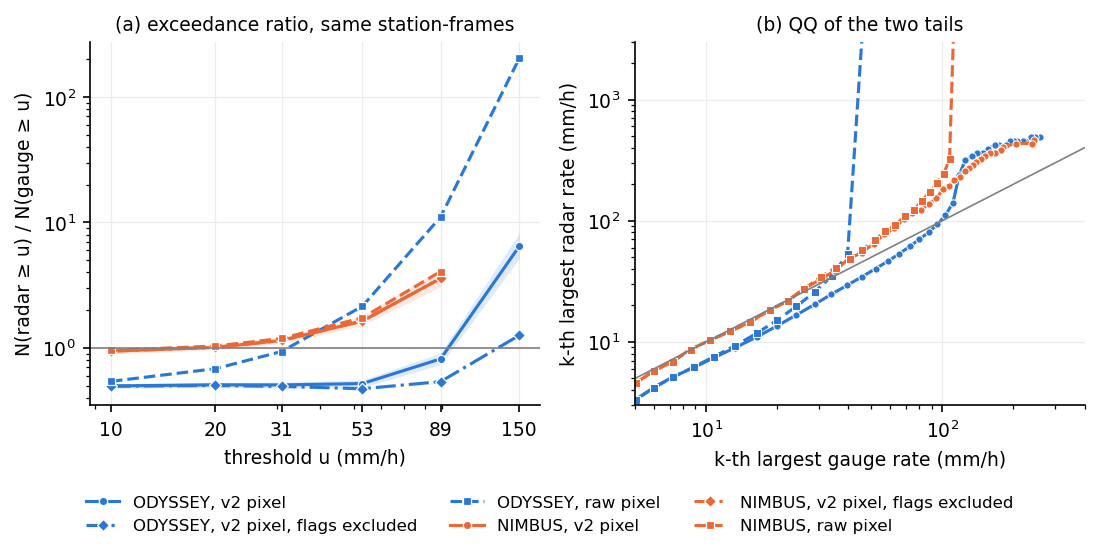
\includegraphics[width=\linewidth]{fig_gauge_values.png}
    \end{column}
    \begin{column}{0.46\textwidth}
      \footnotesize
      \begin{tabular}{lccc}
        \toprule
        $\rho(u)$ & 31 & 89 & 150 \\
        \midrule
        ODYSSEY raw & 0.93 & 11.0 & 204 \\
        ODYSSEY v2 & 0.51 & 0.82 & 6.5 \\
        \quad flags excluded & 0.49 & 0.54 & 1.26 \\
        NIMBUS v2 & 1.14 & 3.58 & 31 \\
        \bottomrule
      \end{tabular}
      \vspace{2mm}

      \begin{itemize}
        \item ODYSSEY exceeds u about half as often as the gauges at every level up to 53\mmh\ (89 with flags excluded): the tail \emph{shape} matches, and u = 31 sits on the calibrated part.
        \item NIMBUS is heavier than the gauges from $\approx$ 31\mmh, and no rule touches it.
        \item At gauge $\ge$ 30\mmh\ the cleaned radar $3\times3$ max is $\ge$ 10\mmh\ in
          71\% of cases; median radar/gauge 0.45.
      \end{itemize}
    \end{column}
  \end{columns}
\end{frame}

% ---------------------------------------------------------------------------
\section{v3: repair instead of reject}

\begin{frame}{v3 rebuild (done 2026-10-05)}
  \small
  \begin{itemize}
    \item \textbf{Repairs replace tile rejection.} Footprints ($\ge$150\mmh\ regions around a
      $>$500 core), ray components, ring pixels $\ge$ 89\mmh, and cells without temporal
      support are lowered to the median of their outer ring.
    \item \textbf{Validated on the same 12.1M gauge pairs.} ODYSSEY $\rho$ at 150\mmh:
      6.46 (v2) $\to$ 1.47 [1.12, 1.92]. Under repaired pixels the gauge saw $\ge$ 10\mmh\ in
      5.3\% of cases (untouched: 44.6\%). NIMBUS unchanged.
    \item Ring repair starts at 89\mmh, not 31: rings at 31--89\mmh\ held real rain (38.5\%
      gauge $\ge$ 10\mmh).
    \item \textbf{Event set fixed}: the 2013 Central European floods and the Andreas
      hailstorms were training days in v2; Emilia-Romagna recovered with shifted windows.
    \item \textbf{Built} in 33\,h on 8 workers: train 1,962,057 / val 252,809 / test 297,460 /
      nimbus 487,673; \code{events\_test} 36,166 tiles of 25 events, \code{events\_nimbus}
      5,249 (Boris, Valencia DANA). All checks passed; min gap between splits 2 days.
  \end{itemize}
\end{frame}

% ---------------------------------------------------------------------------
\section{The POT threshold study exposes three radar failures}

\begin{frame}{No threshold is stable on v3}
  \begin{columns}[T]
    \begin{column}{0.6\textwidth}
      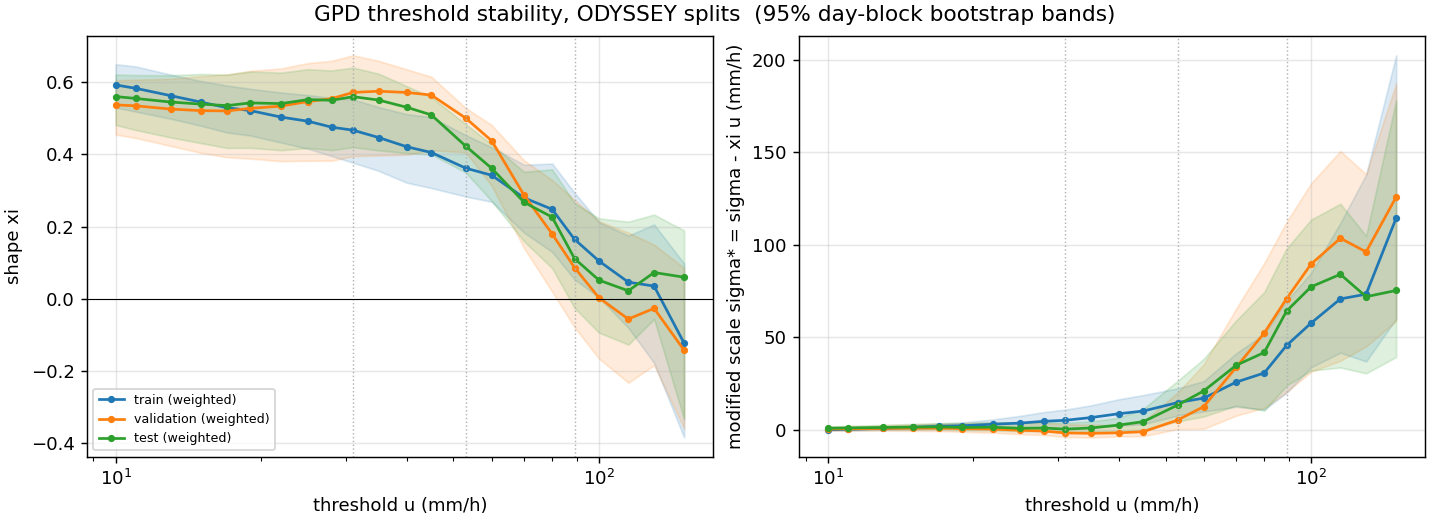
\includegraphics[width=\linewidth]{stability_splits.png}
    \end{column}
    \begin{column}{0.38\textwidth}
      \small
      GPD fits over u = 10--150\mmh, day-block bootstrap (B = 200).
      \vspace{1mm}

      $\xi$ falls monotonically: train +0.47 at 31, +0.17 at 89, $-$0.12 at 150.
      \vspace{1mm}

      Sub-asymptotic shape, or artefacts? The top 10 train days hold 37\% of the exceedances
      of 89\mmh, so look at them.
    \end{column}
  \end{columns}
\end{frame}

\begin{frame}{Two failures shape the v3 tail}
  \centering
  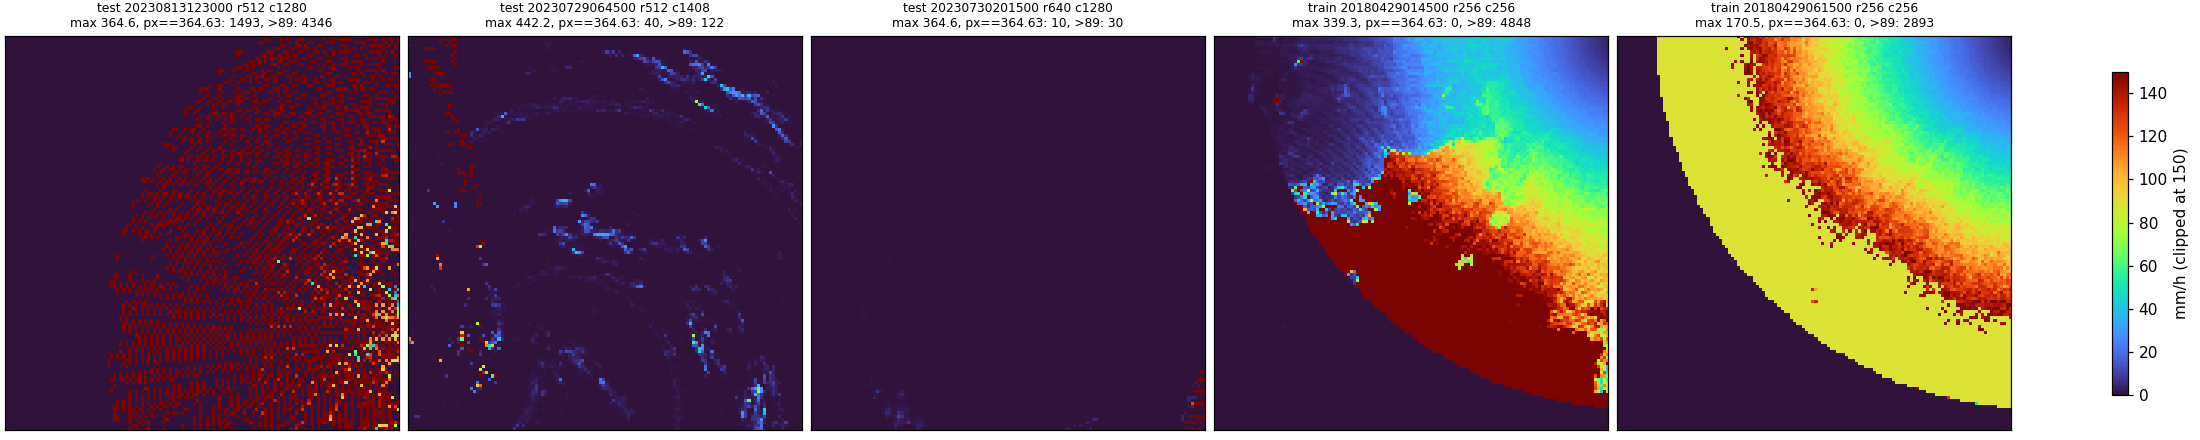
\includegraphics[width=\linewidth]{tail_suspects.png}
  \vspace{1mm}

  \raggedright\small
  \begin{itemize}
    \item \textbf{364.63\mmh\ = 64.0\,dBZ} under $Z = 200R^{1.6}$: a reflectivity ceiling of
      the Valjevo (Serbia) area on 80 rain days of 2023; 12\% of all test pixels $>$89\mmh.
    \item \textbf{Torrejón de Velasco (Madrid), 2018-04-29}: a whole radar disk at a smooth
      range-dependent 60--340\mmh; 16\% of all train exceedances of 89\mmh. The v3 repair
      lowered it to its ring median, which is the same failing radar: a flat 88.27\mmh\
      plateau.
    \item Removing only these tiles (797 of 1.07M train) flattens $\xi(u)$: +0.34 to +0.37 over
      31--89\mmh.
  \end{itemize}
\end{frame}

\begin{frame}{A third failure, found by a repeated-value test}
  \begin{columns}[T]
    \begin{column}{0.55\textwidth}
      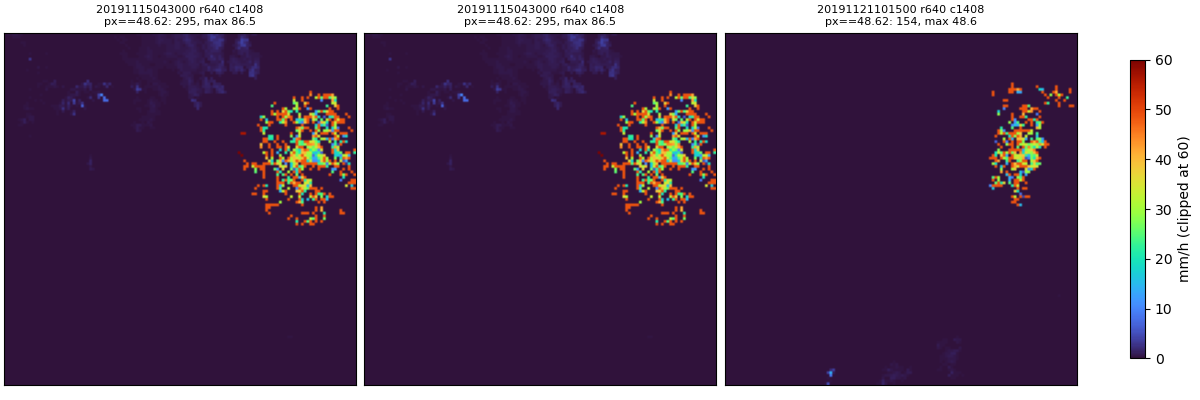
\includegraphics[width=\linewidth]{tail_suspects_4862.png}
    \end{column}
    \begin{column}{0.43\textwidth}
      \small
      Real rain on the 0.01\mmh\ ODYSSEY grid almost never repeats one value: per tail tile,
      median 1 and 99.9th percentile 24 repeats of one value $\ge$ 31\mmh.
      \vspace{2mm}

      $\ge$ 50 repeats flagged 0.069\% of train tail tiles and found \textbf{48.62\mmh\ =
      50.0\,dBZ}, Oradea (Romania), tile r640 c1408, 7 days in November 2019.
      \vspace{2mm}

      Why v3 missed all three: each v3 rule assumes an artefact that is small, local or
      transient. These are large, smooth or persistent.
    \end{column}
  \end{columns}
\end{frame}

% ---------------------------------------------------------------------------
\section{The v4 screen}

\begin{frame}{Five rules, each keyed on an error signature (DECISIONS §19)}
  \small
  \begin{enumerate}
    \item \textbf{Repeated value per tile} ($\ge$ 50 repeats of one value $\ge$ 31\mmh; on
      NIMBUS counted in excess of the adjacent ladder levels).
    \item \textbf{Ceiling table} per radar area and year. A ceiling pixel is censored, not
      measured: $\ge$ 5 per tile-frame $\Rightarrow$ reject; 1--4 $\Rightarrow$ repair like a
      spike.
    \item \textbf{Radar-disk failure} per radar and frame: wet fraction, share of log-rate
      variance explained by range alone, jump at the area boundary and the maximum-range
      circle.
    \item \textbf{Guarded repair}: \code{boundary\_fill} refuses components above a size
      limit; the repeated-value test runs after every repair.
    \item \textbf{Radar-day ranking} against each radar's own seasonal level and its 5 nearest
      radars; exclusions from a list reviewed by eye.
  \end{enumerate}
  \vspace{1mm}
  Policy (DECISIONS §17): reject clear errors only, keep imperfections, no labelled set.
  None of the rules keys on intensity alone; every rule reports its rejection rate by
  intensity bin, because real extremes look anomalous too.
\end{frame}

\begin{frame}{When is the dataset ready? A gate fixed in advance (DECISIONS §20)}
  \small
  Ready when one more cleaning step would not change any number we report.
  \begin{enumerate}
    \item \textbf{Known failures caught}, kept in a regression catalogue.
    \item \textbf{Residual contamination measured}: 100 random test tiles with max $\ge$
      89\mmh\ looked at; 95\% upper bound on the artefact rate $\le$ 5\%.
    \item \textbf{Evaluation reference stable}: dropping the 20 most influential non-event days
      moves no observation-side table number outside its day-block bootstrap interval.
    \item \textbf{Real extremes survive}: $<$ 0.5\% rejected per event; no rule's rejection
      rate climbs steeply with intensity; gauge $\rho$ no worse than v3.
    \item \textbf{Residual drift in $\xi(u)$ explained} (truncation at 500\mmh, mixing,
      sub-asymptotic threshold) with a truncated-GPD fit.
  \end{enumerate}
  \vspace{1mm}
  \textbf{No cleaning by tail fit}: selecting data by its fit to the GPD and then using the
  GPD as evaluation reference would be circular. The fit points at candidates; rules key on a
  ceiling value, a range-only field, a repeated value.
\end{frame}

\begin{frame}{Build plan}
  \small
  \begin{tabular}{lll}
    \toprule
    phase & content & status \\
    \midrule
    1 & code: \code{src/data/radar\_screen.py}, guarded repair, tests & done \\
    0 & calibration on known failures, 27 events, 100 random days & run 2 passed \\
    2 & radar pass over all days, ceiling table, radar-day review list & next ($\sim$9\,h) \\
    3 & tile scan with the v4 chain & ($\sim$12\,h) \\
    4 & store, gamma targets, checks & ($\sim$20\,h) \\
    5 & audit = the §20 gate & \\
    \bottomrule
  \end{tabular}
  \vspace{2mm}

  Decisions are taken at split time from per-tile columns, so a threshold can change without
  a rescan. Retraining starts only after the gate.
\end{frame}

% ---------------------------------------------------------------------------
\section{Phase 0: calibration}

\begin{frame}{Run 1 failed on the ceiling rule}
  \small
  First rule 2: a value counted $>$ 50$\times$ the median of its occupied $\pm$0.5\,dB
  neighbours.
  \begin{itemize}
    \item \textbf{3,256 radar-year ``ceilings''} where a real ceiling is one value. Event gate
      failed entirely through rule 2: valencia\_dana 100\%, ce\_floods 93\%, boris 93\%
      of wet tiles rejected.
    \item Cause: a radar-year mixes values on coarse ladders (dBZ steps of 0.4--3\,dB) with
      sparse off-ladder values (counts 1--4). The median of the neighbours is then $\approx$1
      and every ladder level passes. Example: Málaga 2024, 10.28\mmh\ counted 8,059 times
      among neighbours counted 1--4.
  \end{itemize}
  \vspace{1mm}
  \textbf{New comparison:} the count of a value against the \emph{largest} count of any other
  value within $\pm$4\,dB (wider than the coarsest ladder step, $\approx$3\,dB). Rain counts
  fall with intensity, so on a ladder the ratio is $\lesssim$1; a ceiling piles up above its
  neighbours.
  \begin{itemize}
    \item Calibration (199 days, 23,868 values counted $\ge$ 50): the 18 rows of the two known
      ceilings score 9.9--89; all other values have 99.9th percentile 1.96.
      $\Rightarrow$ \code{min\_ratio: 5} (provisional).
  \end{itemize}
\end{frame}

\begin{frame}{Run 2: gates}
  \small
  \textbf{Ceiling table: 21 rows.} 364.63\mmh\ on 17 radar-years (Serbia, Croatia,
  Thessaloniki, Brindisi), 48.62\mmh\ Oradea 2019, and 11.53\mmh\ = 40.0\,dBZ on three of the
  same Balkan radars in 2023.
  \vspace{2mm}

  \begin{tabular}{lcc}
    \toprule
    Gate 1: known failures & tiles & caught \\
    \midrule
    Madrid 2018-04-29, $\ge$ 10\% Madrid-owned, max $\ge$ 31 & 101 & 96 \\
    364.63 (2023) and 48.62 (2019) in the ceiling table & 2 & 2 \\
    48.62 days, tile r640 c1408, max $\ge$ 31 & 411 & 310 \\
    \bottomrule
  \end{tabular}
  \vspace{2mm}

  \textbf{Gate 2 passed:} worst event 0.14\% rejected (chauxdefonds, 1 tile, rule 1); 24 of 25
  events 0\%. Random days: rejection $\le$ 0.014\% below 150\mmh, 0.74\% at $\ge$ 150\mmh\
  (Valjevo-area tiles). All 110 tiles with max $>$ 500\mmh\ are rejected.
  \vspace{1mm}

  \textbf{Regression:} with v4 switched off, 2018-06-15 reproduces the v3 table.
\end{frame}

\begin{frame}{Rule 3: the radar-disk failure separates cleanly}
  \begin{columns}[T]
    \begin{column}{0.62\textwidth}
      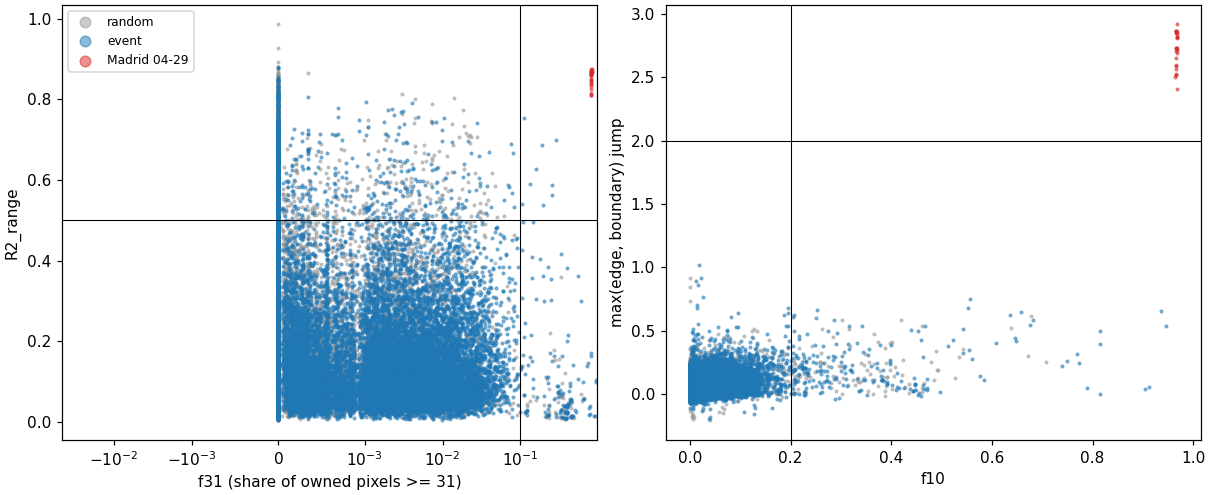
\includegraphics[width=\linewidth]{radar_frames.png}
    \end{column}
    \begin{column}{0.36\textwidth}
      \small
      Per radar and frame (wet frames, wet fraction $\ge$ 0.2):
      \vspace{1mm}

      Madrid 04-29 frames: share $\ge$ 31\mmh\ 0.82, $R^2$ of log-rate on range 0.86, jump
      2.4--2.9.
      \vspace{1mm}

      Random and event frames: edge jump 99.9th percentile 0.10--0.14, boundary jump 0.38--0.48; largest jump of either 1.02.
      \vspace{1mm}

      22 other flagged radar-frames on 13 radar-days, mostly the 2023 Balkan radars.
    \end{column}
  \end{columns}
\end{frame}

% ---------------------------------------------------------------------------
\section{Gallery review (7 October)}

\begin{frame}{The rule galleries are dominated by one failure}
  \centering
  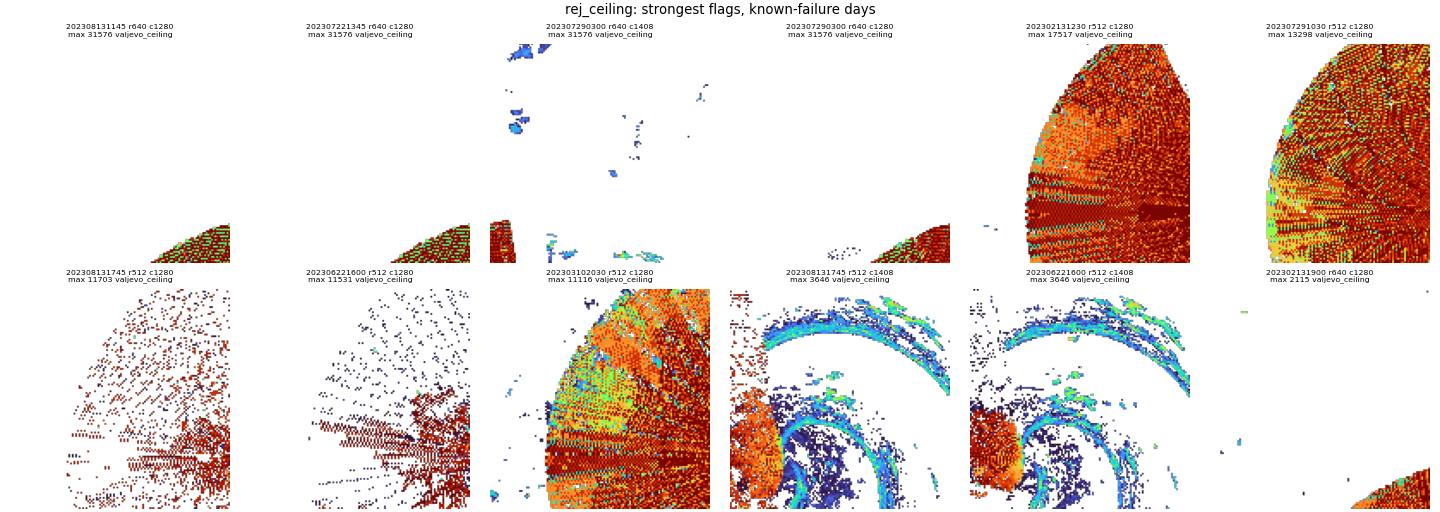
\includegraphics[width=0.92\linewidth]{gallery_rej_ceiling_tp.png}
  \vspace{1mm}

  \raggedright\small
  The galleries show each rule's 12 strongest flags by tile max. All of them come from the 2023
  Balkan failure; the ``random / event'' panels fall inside its window (02-13 to 08-13), so they
  are true positives too. Every panel is visibly broken: spokes, saturated sectors, speckle.
  The open Gate-1 questions need galleries targeted on them.
\end{frame}

\begin{frame}{Madrid: the five kept tiles are outside the failure}
  \centering
  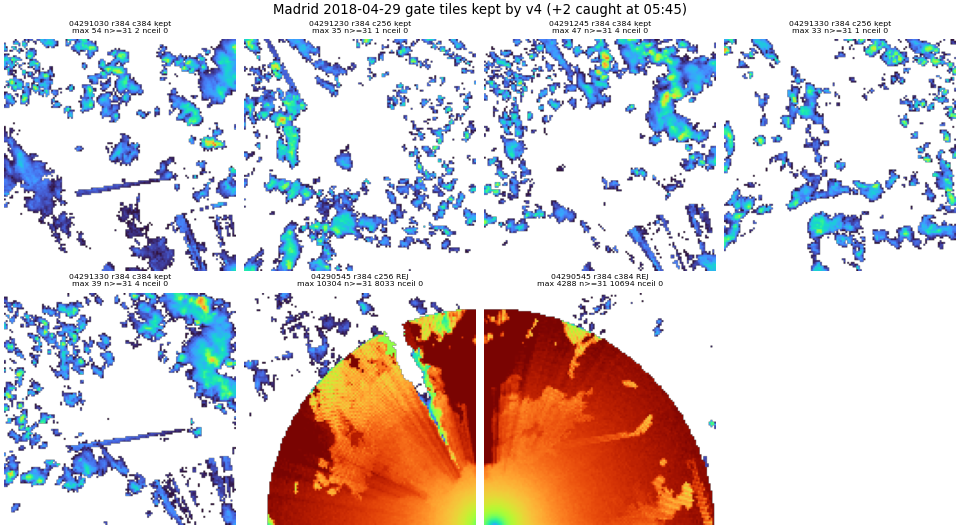
\includegraphics[width=0.78\linewidth]{madrid_kept.png}
  \vspace{1mm}

  \raggedright\small
  All 96 gate tiles in the failure window (00--06\,h) are rejected. The 5 kept tiles are from
  10:30--13:30, max 33--54\mmh, scattered convection; the two right-hand panels show the same
  tiles at 05:45. \textbf{Closed.}
\end{frame}

\begin{frame}{48.62: the ceiling is handled, a second failure is not}
  \centering
  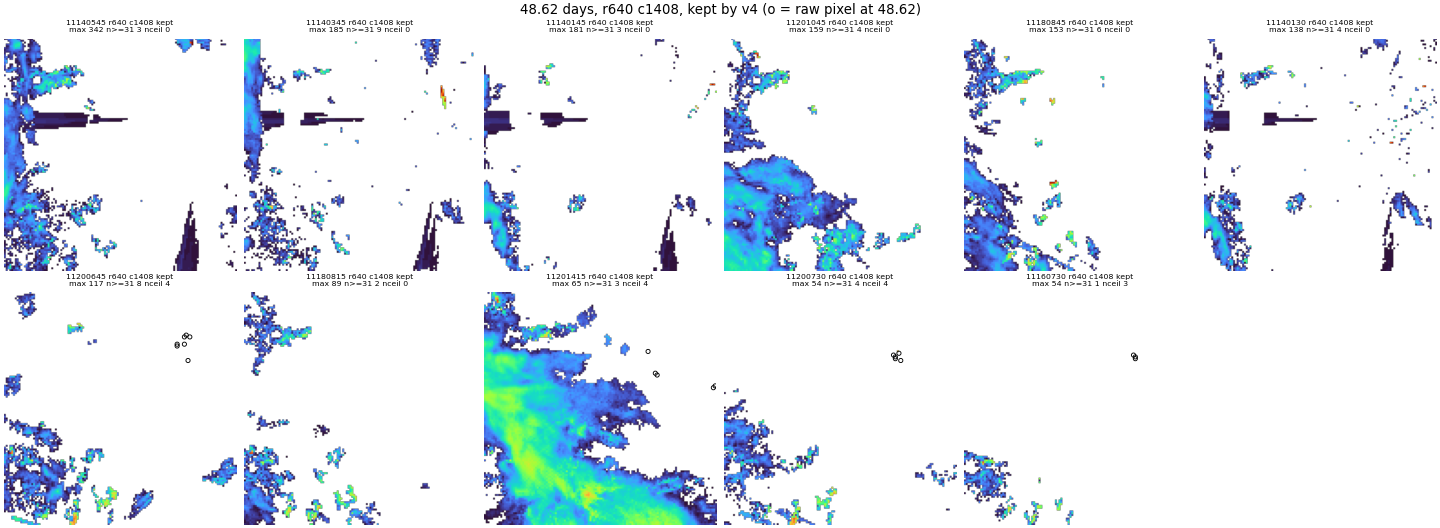
\includegraphics[width=\linewidth]{c4862_kept.png}
  \vspace{1mm}

  \raggedright\small
  Kept frames carry 0--4 raw 48.62 pixels (circles), repaired as designed. But their maxima
  (138--342\mmh) are clusters of 2--9 pixels whose $5\times5$ median (10\,km) is 0\mmh. The
  repair can copy such values: 5,524.7 $\to$ 153.4\mmh\ from an equally isolated neighbour.
\end{frame}

\begin{frame}{Two smaller findings}
  \small
  \textbf{11.53\mmh\ (40.0\,dBZ), 2023.} 398 pixels in total on three radars (grthe, rsfrg,
  itbri). Its largest days (02-14, 06-11, 07-12, 07-22, 07-29) are all 364.63 failure days,
  so it is probably the same fault; the calibration set over-samples those days, so the link
  is weak. It only triggers repairs (no tile below 89\mmh\ is rejected for a ceiling).
  Kept flagged.
  \vspace{3mm}

  \textbf{Refused repairs on real rain.} Three tiles rejected because the guard refused a
  repair look like ordinary frontal bands (max 30--40\mmh). Rate on random days
  $\le 1.4\times10^{-4}$ per intensity bin; still to check what was refused.
  \vspace{2mm}

  \centering
  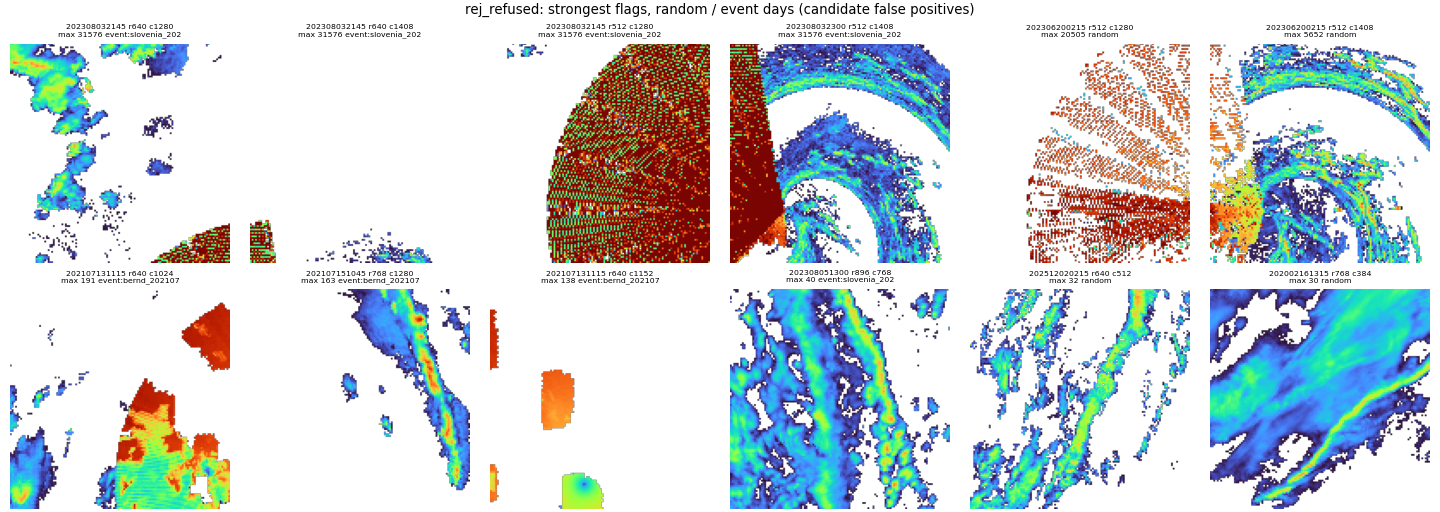
\includegraphics[width=0.62\linewidth]{gallery_rej_refused_fp.png}
\end{frame}

% ---------------------------------------------------------------------------
\section{Isolated high values}

\begin{frame}{Isolated high values: how often, and where?}
  \centering
  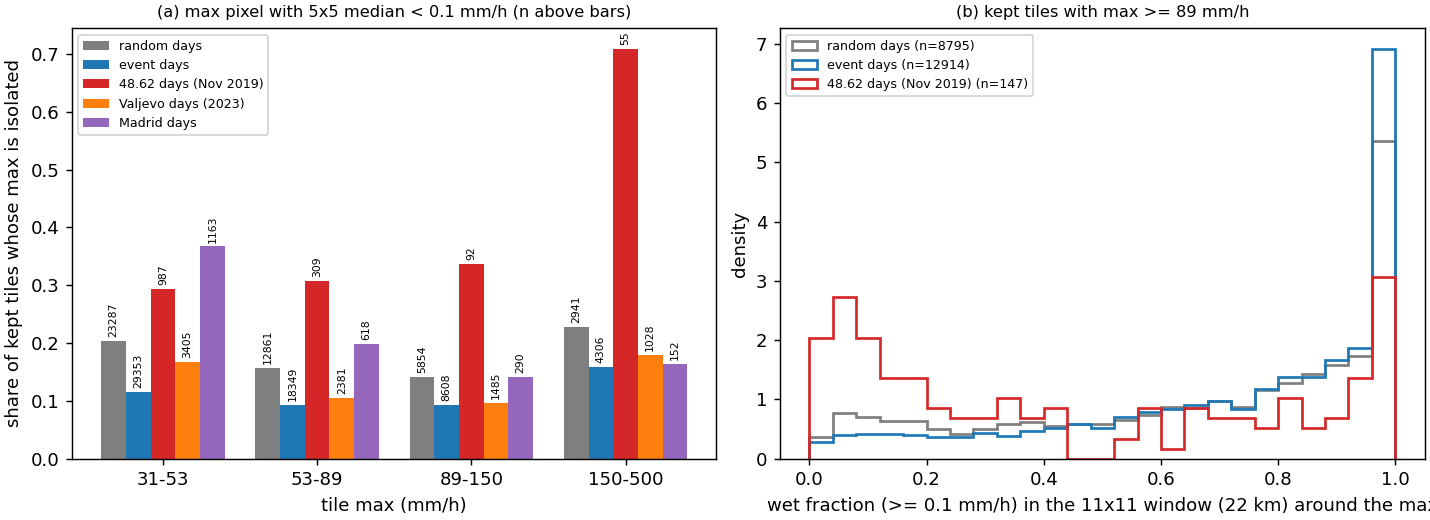
\includegraphics[width=0.86\linewidth]{isolated.png}
  \vspace{1mm}

  \raggedright\small
  Phase-0 days, 118,627 tiles with max $\ge$ 31\mmh, v4-cleaned field
  (\code{scripts/dataset\_v2/isolated\_v4.py}). A pixel is isolated when the median of its
  $5\times5$ window (10\,km) is $<$ 0.1\mmh\ and the window is $\ge$ 50\% covered.
\end{frame}

\begin{frame}{Isolation alone is not a clear-error signature}
  \small
  \begin{itemize}
    \item On the 48.62 days the max is isolated far more often: 71\% of kept tiles at
      150--500\mmh, against 16\% on event days and 23\% on random days.
    \item \textbf{But the event days show it too}: 9--16\% of kept event tiles have an
      isolated max, in every intensity bin.
    \item The strictest cut tried (wet fraction $<$ 0.05 in the $11\times11$ window, 22\,km)
      still flags 1.8\% of event tiles with max $\ge$ 89\mmh, against 15.6\% on the 48.62 days
      and 2.7\% on random days. Gate 2 allows $<$ 0.5\% per event.
    \item Whether the isolated event maxima are small real cells or artefacts inside event
      windows is not known; they have not been looked at.
  \end{itemize}
  \vspace{2mm}
  \textbf{Reading:} a per-tile isolation rule would remove real storms at several times the
  gate rate (DECISIONS §17, safeguard 1). The 48.62 days stand out by \emph{rate}, which is a
  radar-day property. The natural home is rule 5 (radar-day ranking): the share of isolated
  maxima per radar and day, against the radar's own level and its neighbours.
\end{frame}

\begin{frame}{Rule 5 gains a signal: isolated high pixels per radar-day}
  \small
  $\text{iso31}$ = owned pixels $\ge$ 31\mmh\ with an isolated $5\times5$ window, summed over the
  day, on the field before the v3 repairs. Scored like the other signals:
  \[
    \text{score} = \log_{10}\frac{x + f}{\max\left(q_{99}^{\text{own, season}},\;
      \text{median}_{\text{5 nearest radars}}\right) + f}, \qquad f = 10 \text{ pixels}
  \]
  A radar-day only enters the review list; nothing is removed without a look.
  \vspace{2mm}

  \footnotesize
  \centering
  \begin{tabular}{lrrrr}
    \toprule
    Oradea, Nov 2019 & iso31 & neighbour median & own autumn $q_{99}$ & score \\
    \midrule
    11-14 & 8,636 & 0 & 7,525 & +0.06 \\
    11-18 & 6,500 & 2 & 7,525 & $-$0.06 \\
    11-17 (weakest) & 1,286 & 2 & 7,525 & $-$0.76 \\
    \bottomrule
  \end{tabular}
  \vspace{2mm}

  \raggedright\small
  Phase-0 check (199 days): the signal is strong against the neighbours, but 7 of Oradea's 53
  autumn days in the calibration set are failure days, so its own $q_{99}$ is a failure day.
  On the full archive they are $<$ 1\% of $\approx$1,180 days. Event radar-days: 232 of 15,897
  score $>$ 0, none $\ge$ 0.5. Rule-3 flags unchanged.
  \vspace{1mm}

  \textbf{Open:} a radar failing on more than $\approx$1\% of its season-days hides behind its
  own $q_{99}$. Own $q_{90}$ or neighbours only, decided on the full-archive ranking (no rescan).
\end{frame}

\begin{frame}{A by-product: 486.2\mmh\ = 66.0\,dBZ}
  \small
  \begin{itemize}
    \item 55 tiles have a max of exactly 486.2\mmh; no other value between 470 and 500\mmh\
      is the max of more than 3 tiles.
    \item 486.2\mmh\ is 66.0\,dBZ under $Z = 200R^{1.6}$, the same kind of round reflectivity
      value as 364.63 (64.0\,dBZ) and 48.62 (50.0\,dBZ).
    \item 36 of the 55 tiles are on event days, 15 random, 4 Valjevo; it is also the v3 maximum
      of both NIMBUS events (Boris, Valencia DANA).
    \item It is not in the ceiling table: per radar-year it is too rare for
      \code{min\_count: 50} or does not pile up 5$\times$ above its neighbours.
  \end{itemize}
  \vspace{2mm}
  \textbf{Likely explanation: our bound, not the product.} On data in 0.5\,dBZ steps the levels
  are 65.0, 65.5, 66.0, 66.5\,dBZ = 421.1, 452.5, 486.3, 522.6\mmh: 66.0\,dBZ is the highest level
  below 500\mmh, and 66.5 is repaired. So these radars are censored at 486\mmh\ by the bound,
  and their maxima pile up there. Seen once directly: an artefact arc (2014-06-08 06:45) whose
  leftovers after repair are exactly 486.2, 452.5, 421.1 and 391.8\mmh. Which of the 55 tiles
  are artefacts and which are real cores is not checked.
\end{frame}


% ---------------------------------------------------------------------------
\section{Open items and next steps}

\begin{frame}{Open items}
  \small
  \begin{itemize}
    \item \textbf{Isolated maxima}: no tile-level rule. Decide whether to add the share of
      isolated maxima per radar-day to rule 5; it must go into the radar pass before Phase 2.
    \item \textbf{486.2\mmh}: product cap or radar fault? Read from the Phase-2 histograms.
    \item Commit the rule-2 change; launch Phase 2 (radar pass, $\sim$9\,h, all 8 cores).
    \item Review the radar-day list by eye; record exclusions in \code{quality\_v4.yaml}.
    \item Phases 3--5 ($\sim$32\,h of compute), then the §20 gate.
    \item Re-derive the POT threshold on v4 (\code{pot\_threshold.py --version v4}), with a
      truncated GPD.
    \item NIMBUS tail excess over the gauges: test with DWD 1-min records.
    \item Re-run the ring-repair gauge validation at 89\mmh\ (it was run at 31).
    \item Archive fetch 2025-10-23 to 2026-09-22 (334 days), blocked by quota.
    \item Talk to MeteoSwiss (D.\ Nerini, L.\ Moret) on filters, plausibility bounds and
      o.o.d.\ test design.
  \end{itemize}
\end{frame}

\begin{frame}{Known limits of the dataset}
  \small
  \begin{itemize}
    \item Tiles need 100\% radar coverage: coastal and network-edge extremes (Mediterranean)
      are under-represented; HyMeX IOP16 is absent from the archive.
    \item Radar rates underestimate intense rain (at gauge $\ge$ 30\mmh\ the median radar/gauge ratio is 0.45;
      Valencia: 28.6\mmh\ radar pixel vs a 184.6\mmh\ gauge-hour at Turís).
    \item NIMBUS evaluation carries a product penalty (small-scale variance, persistence,
      heavier tail) unrelated to extremeness; report it against a same-product reference.
    \item The data are truncated at 500\mmh\ after repair; a truncation alone makes $\xi$ fall at
      high u.
    \item No labelled set: precision and recall of the rules on real extremes are bounded by
      the gallery review, the per-bin rates and the gauges, not measured.
  \end{itemize}
\end{frame}

\end{document}
